\chapter[Escopo]{Escopo}

\section{Objetivo do projeto}
Desenvolver um sistema anticolisão veicular que alerte o motorista sobre ultrapassagens potencialmente perigosas, contra veículos que estejam vindo em direção contrária.
O sistema não terá autonomia sobre o veículo em questão, apenas terá a finalidade de alertar se a manobra será segura ou não.

\section{O que vai ser feito}
Um Sistema Interveicular de Alerta Anti-colisão de Veículos em rodovias brasileiras (SIAAV).

\section{Clientes Do Sistema}
O sistema atenderá motoristas de veículos automotores, que seguem as normas do Código de Trânsito brasileiro e trafegam por rodovias brasileiras.

\section{Onde o sistema Funcionará}
Visto que no Brasil dos 188.925 acidentes em rodovias, 7.008 causaram mortes e 63.980 deixaram pessoas feridas em 2011, segundo o DNIT, o sistema visa o uso nas rodovias a fim de reduzir esses números. \cite{ministerio}

\section{Velocidade Máxima}
Foi definido, conforme o Código de Trânsito Brasileiro \cite{ctb}, que a velocidade máxima de operação do equipamento é de 110km/h.
Esta velocidade será referência para cálculos futuros sobre Distância Máxima.

\section{Distância de Visibilidade de Ultrapassagem}
De acordo com a Norma de Traçado (JAE P3/94) é considerado que a distância  de ultrapassagem pode ser obtida empiricamente através da expressão:

$DU = 7*VT$
\begin{itemize}
  \item DU - Distância de Ultrapassagem.
  \item VT - Velocidade de Tráfego ( ou relativa )
\end{itemize}

Esse cálculo garante a 85\% dos condutores a Distância de Visibilidade, que é a distância mínima para que um motorista ultrapasse um outro veículo em segurança e sem forçá-lo a reduzir sua velocidade. \cite{costa}

Os cálculos para tomada de decisão do sistema serão baseados, entre outros, nas seguintes características:

\begin{itemize}
  \item Velocidade do veículo que iniciou a ultrapassagem;
  \item Velocidade do veículo a ser ultrapassado;
  \item Velocidade do veículo que trafega no sentido contrário.
\end{itemize}

Outras relações de Velocidade e Distância estão na tabela abaixo:
\begin{figure}[h]
  \centering
  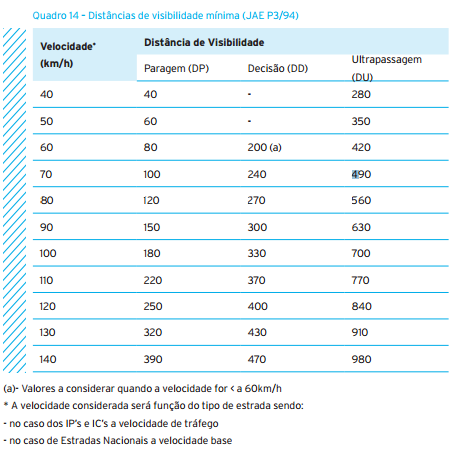
\includegraphics[width=330px, scale=0.5]{figuras/visibilidade}
  \caption{Relação de velocidade e distância segura para ultrapassagem}
  \label{fig:visibilidade}
\end{figure}

\section{Distância mínima até o veículo a frente}
Utilizando os dados fornecidos na figura \ref{fig:visibilidade}, podemos definir a distância mínima de segurança, assumindo que o veículo esteja a uma velocidade máxima de 110km/h, de 264 metros. Esta distância tem como base a Distância de Visibilidade para Paragem (DP), acrescidos 20\% para margem de segurança.

\section{Tempo de resposta dos aparelhos empregados no sistema}
\begin{itemize}
  \item Sensor MFC \cite{mfc} : < 10 ms.
  \item Trânsponder VDL 4000/VTE: 3,0 ms.
\end{itemize}

\section {5W2H}

\subsection{O que será feito}
Será Construido um sistema anticolisão veícular que alerto o motorista sobre ultrapassagens potencialmente perigosas contra veículos que estejam vindo em direção contrária. O sistema não terá autonomia sobre os comandos do veículo, apenas terá a finalidade de alertar se a manobra é segura ou nao.

\subsection{Porque será feito}
Foi observado que no Brasil há um número muito alto de acidentes com ferimentos ou mortes. 188.925 acidentes em rodovias, das quais 7.008 causaram mortes e 63.980 deixaram pessoas feridas em 2011, segundo o DNIT [4]. Sendo assim o projeto visa construir um sistema que diminua o percentual de acidentes.

\subsection{Onde será feito}
UnB-Fga

\subsection{Quando será feito}
O Cronograma do primeiro ponto de controle está disponível na Figura \ref{fig:1cronograma} dos Apêndices

\subsection{Por quem será feito}
Pela Equipe 5 da matéria de Projeto integrador 1. A equipe é composta por diversos estudantes de Engenharia do campus FGA

\begin{description}
  \item[Engenharia de Energia] \hfill
  \\Vinicius Ciurlini
  \\Alessandro Alcantara
  \\Tainara Costa
  \item[Engenharia de Software] \hfill
  \\Igor Ribeiro
  \\Vinicius Bandeira
  \\Tiago Ribeiro de Assunção
  \\Marcelo Herton
  \\Luis Henrique
  \\João Henrique
  \\Igor Ribeiro
  \\Wilton Rodrigues
  \\Gustavo Sabino
  \item[Engenharia Eletrônica] \hfill
  \\Dario Descartes
  \\Fernanda Cosme
  \\Lucas Luan
  \\Carol Miedazis
  \item[Engenharia Automotiva] \hfill
  \\Renato Lucas Carvalho
  \\Khatarinne
  \item[Engenharia Aeroespacial] \hfill
  \\Brenno Taylor de Jesus Popov
\end{description}

\subsection{Como será feito}
Por meio de pesquisas sobre acidentes em estradas brasileiras, comparações com tecnologias já empregadas ou tecnologias em desenvolvimento,  análise técnica de equipamentos avulsos como transpônder, GPS,  sensores, análise de viabilidade técnica, análises sobre a estrutura dos veículos candidatos ao porte do equipamento, consultas a legislação brasileira.
